\documentclass[a4paper, 10pt]{article}%тип документа
\usepackage[T2A]{fontenc} %кодировка
\usepackage[utf8]{inputenc} %кодировка исходного кода
\usepackage[english,russian]{babel} %локализация и переносы
\usepackage{multirow}
\usepackage{wrapfig}
\usepackage{graphicx}
\usepackage{mathtext}
\usepackage{amsmath}
\usepackage{siunitx} % Required for alignment
\usepackage{multirow}
\usepackage{rotating}
\usepackage{float}
\usepackage[T1,T2A]{fontenc}
\usepackage[russian]{babel}
\graphicspath{{pictures/}}
%Производные
\usepackage{physics}
%Математика
\usepackage{amsmath, amsfonts, amssymb, amsthm, mathtools}
\usepackage[left=10mm, top=20mm, right=18mm, bottom=15mm, footskip=10mm]{geometry}
\title{1.4.2 Определение ускорения свободного падения при помощи оборотного маятника}
\author{Мыздриков Иван, Б06-401}
\date{23 октября 2024 г.}

\begin{document}

\maketitle

\section{Аннотация}
Цель работы: с помощью оборотного маятника измерить величину ускорения свободного падения. 

В работе используются: оборотный маятник с двумя подвесными призмами и двумя грузами (чечевицами); электронный счётчик времени и числа колебаний; подставка с острием для определения положения центра масс маятника; закреплённая на стене консоль для подвешивания маятника; металлические линейки, штангенциркуль длиной 1 м. 

\section{Теоретические сведения}
При малых колебаниях период колебаний физического маятника определяется формулой:

\[T = 2 \pi \sqrt{\frac{J}{mgl}}\]
Где J - момент инерции маятника относительно оси качания, m - масса маятника, l - расстояние от оси качания до центра масс маятника. 
Если сравнить это выражение с известной формулой колебаний математического маятника длиной l ($T = 2 \pi \sqrt{\frac{l}{g}}$), можно определить приведённую длину физического маятника как 
\[l_\text{пр} = \frac{J}{ml}\]
Смысл приведённой длины в том, что при длине математического маятника, равной $l_\text{пр}$, его период колебаний совпадает с периодом колебаний физического маятника. 
Теорема Гюйгенса об оборотном маятнике 
Пусть $O_1$ — точка подвеса физического маятника, а C — его центр масс. Отложим отрезок длиной $l_\text{пр}$ вдоль линии $O_1 C$, и обозначим соответствующую точку как $O_2$ — эту точку называют центром качания физического маятника. Заметим, что приведённая длина всегда больше расстояния до центра масс ($l_\text{пр} > l$), поэтому точка $O_2$ лежит по другую сторону от центра масс. 
Точки $O_1$ и $O_2$ обладают свойством взаимности: если перевернуть маятник и подвесить его за точку $O_2$, то его период малых колебаний останется таким же, как и при подвешивании за точку $O_1$ (теорема Гюйгенса). На этом свойстве — «оборотности» — и основан довольно точный метод определения ускорения свободного падения, применяемый в данной работе. 
Докажем теорему Гюйгенса об оборотном маятнике. Пусть $O_1$ и $O_2$ — две точки подвеса физического маятника, лежащие на одной прямой с точкой C по разные стороны от неё. Тогда периоды колебаний маятника равны соответственно  
\[T_1 = 2 \pi \sqrt{\frac{J_1}{mgl_1}}, T_2 = 2 \pi \sqrt{\frac{J_2}{mgl_2}}\]
По теореме Гюйгенса-Штейнера имеем:
\[J_1 = J_\text{c} + m{l_1}^2 ,J_2 = J_\text{c} + m{l_2}^2 \]
где $J_\text{c}$ — момент инерции маятника относительно оси, проходящей через центр масс перпендикулярно плоскости качания. 
Пусть периоды колебаний одинаковы: $T_1$ = $T_2$ . Тогда одинаковы должны быть и приведённые длины: 
\[l_\text{пр} = \frac{J_1}{ml_1} = \frac{J_2}{ml_2}\]
С учетом выраженных по теореме Гюйгенса-Штейнера моментов инерции получим:
\[l_\text{пр} = l_1 + l_2\]
Таким образом, если периоды колебаний при подвешивании маятника в точках $O_1$ и $O_2$ равны, то расстояние между точками подвеса равно приведённой длине маятника. Нетрудно видеть, что и обратное утверждение также верно. 
Заметим также, что период колебаний маятника, рассматриваемый как функция от $l_1$, $T = 2 \pi \sqrt{\frac{J_\text{c} + m{l_1}^2}{mgl_1}}$ имеет минимум при $l_{1\text{min}} = \frac{J_\text{c}}{m}$. Из (6) видно, что в этой точке $l_1 = l_2 = \frac{l_\textbf{пр}}{2}$, то есть центр масс находится посередине между сопряжёнными точками $O_1$ и $O_2$. 
\begin{figure}
    \centering
    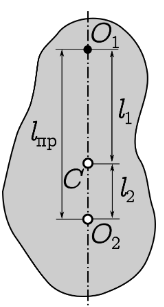
\includegraphics[width=0.15\linewidth]{pic1.png}
    \caption{К теореме Гюйгенса-Штейнера}
    \label{fig:enter-label}
\end{figure}
\section{Методика измерений} %удачиииии ахаххах спасибо
Применяемые в работе маятники представляет собой стержни цилиндрического или прямоугольного сечения длиной ~1 м и массой ∼ 1 ÷ 1,5 кг. Маятник подвешивается с помощью небольших треугольных призм
(П1 и П2), острым основанием опирающихся на закреплённую на стене консоль. Ребро призмы задаёт ось качания маятника. На стержне закрепляются
два дополнительных груза в форме «чечевицы» (Г1 и Г2). Для выполнения
условия I1  > I2 за внешнюю чечевицу Г2 следует крепить за призмой П2, а чечевицу Г1 (внутреннюю) — между призмами П1 и П2 (рис. 2)


\begin{figure}[h]
    \centering
    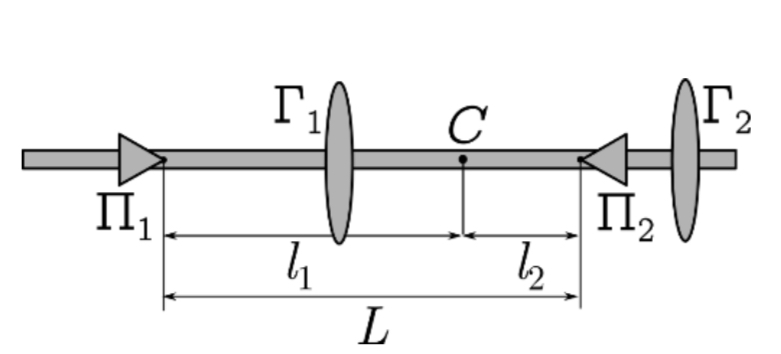
\includegraphics[width=0.35\textwidth]{IMG_1595.jpeg}
    \caption{Схема экспериментальной установки Маятник с грузами}
    \label{fig:mesh1}
\end{figure}


Регистрация времени колебаний проводится с помощью электронных счётчиков. Расстояния между точками установки маятников на консоли до электронных счётчиков фиксировано. Это накладывает ограничения на расположение призм и грузов на стержне. Призмы крепятся симметрично на равном расстоянии от концов стержней так, чтобы маятник при колебаниях пересекал фотоприёмники счётчика, не задевая оправу счётчика.
Фиксированное положение призм однозначно задаёт приведённую
длину оборотного маятника Iпр = L. Изменять в опыте можно только полoжения грузов на стрежне. Главная задача опыта — подобрать такое поло-жение грузов, при котором периоды колебаний при перевороте маятника совпадали бы с достаточно высокой точностью, а для положения центра масс маятника выполнялось при этом условие I1 > 2.5 I2
\paragraph{Действия, которые небоходимо сделать в ходе работы:}
\begin{enumerate}
    \item Взвесьте маятник, его призмы и грузы. Оцените погрешность
    \item Закрепите подвесные призмы симметрично на стержне (положения
призм указаны на установке). Убедитесь, что ребра призм параллельны
друг другу и «смотрят» в сторону центра маятника.
\item Измерьте расстояние  между призмами. Оцените погрешность измерения длины.
\item Задавшись некоторым значением I1/I2 , удовлетворяющим условию
I1 > 2.5 I2, рассчитайте по одной из методик, описанных в Приложении 1,
положения грузов («чечевиц») на стержне. Закрепите их на соответствующих местах.
\item С помощью ⊥-образной подставки определите положение центра масс
маятника с грузами
\item Подвесьте маятник на консоли на призме П2. Включите электронный
счётчик и убедитесь в работоспособности системы (маятник при кача-
нии не касается элементов установки и не проскальзывает в подвесе,
счётчик корректно считает количество колебаний и их время).
\item Проведите измерение времени n = 20 колебаний 3–4 раза, вязкий раз
отклоняя маятник на малый угол  \approx 5 градусов. 
\item Cравните Т1 и Т2, измерьте погрешность




\end{enumerate}

\section{Используемое оборудование}
В работе используются: Оборотный маятник с двумя подвесными призмами и
двумя грузами (чечевицами); электронный счётчик времени и числа колебаний;
подставка с острием для определения положения центра масс маятника; закреплённая на стене консоль для подвешивания маятника; металлические линейки, штангенциркуль длиной 1 м.

Оценка погрешностей измерений:
Мы будем считать по формуле $g_0 = (2 \pi)^2 \frac{L}{T^2}$, поэтому будем считать относительную погрешность косвенных измерений по следующей формуле:

\[\frac{\sigma_{g_0}}{g_0} = \sqrt{(\frac{\sigma_L}{L})^2 + 4(\frac{\sigma_T}{T})^2}\]
Это основная погрешность опыта, для ее минимизации необходимо максимально точно измерить период и расстояние между точками подвеса.
Понятно, что совершенно точно g мы не померяем (из-за различий в измеренных периодах), поэтому нужно посчитать погрешность поправки $\Delta g$.

\[\Delta g \approx 2 \frac{l_2}{l_1 - l_2} \frac{\Delta T}{T} g_0 \]
Тогда если написать выражение для погрешности $\Delta g$ и сложить его с выражением для погрешности $g_0$, получим выражение полной погрешности:

\[\frac{\sigma_g}{g} = \sqrt{(\frac{\sigma_L}{L})^2 + 4(1+2\beta)(\frac{\sigma_T}{T})^2 + 8(\beta \frac{\Delta T \sigma_l}{T \Delta l})^2}\]
Полная относительная погрешность будет равна примерно 0.1, если $\beta < 3/2, \Delta T/T \approx 10^{-2}, \sigma_l/l \approx 10^{-2}$.

\section{Результаты измерений и обработка данных}
Используя таблицу Excel получим нужные нам данные

b1=23,7см

b2=10см

l1=37,4см

l2=14,9см

Jст=0,162 кг*м^2


J=0,319 кг*м^2

Данные,которые мы получили при помощи линейки и весов 

m_{\text{г1}} =1495,4 \text{г}

m_{\text{г2}} =1481,3 \text{г}

m_{\text{п1}} =77,2 \text{г}

m_{\text{п2}} =76,7 \text{г}

m_{\text{ст}} =891,3 \text{г}

l=49см

l=100,4см



Построим график зависимости момента инерции от положения грузов

\begin{figure}[h!]
    \centering
    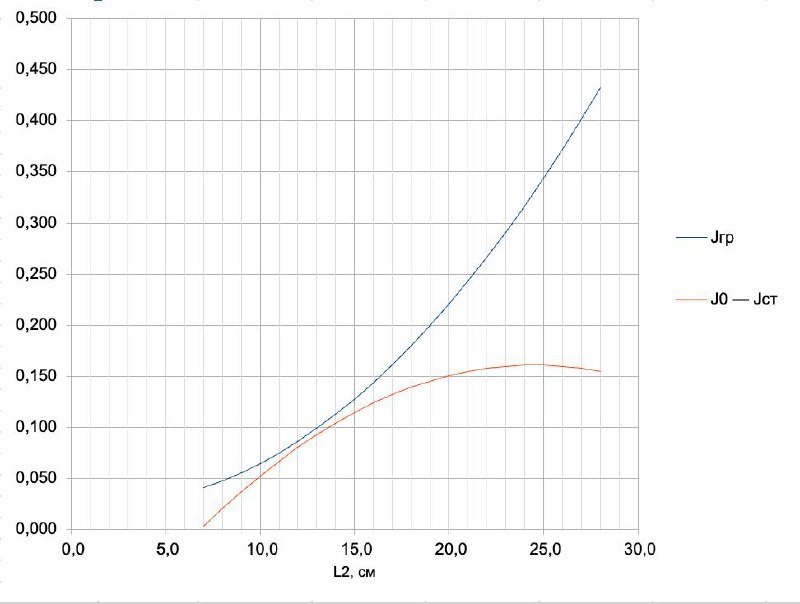
\includegraphics[width=0.15\linewidth]{зависимость.png}
    \caption{Зависимость моментов инерции от длины L2}
    \label{fig:enter-label}
\end{figure}

Найдём погрешности

\[\frac{\sigma_{g_0}}{g_0} = \sqrt{(\frac{\sigma_L}{L})^2 + 4(\frac{\sigma_T}{T})^2} = 0.016 \text{м}/c^2 \]

\[\Delta g \approx 2 \frac{l_2}{l_1 - l_2} \frac{\Delta T}{T} g_0 = 0,084 \text{м}/c^2 \] 

\[\frac{\sigma_g}{g} = \sqrt{(\frac{\sigma_L}{L})^2 + 4(1+2\beta)(\frac{\sigma_T}{T})^2 + 8(\beta \frac{\Delta T \sigma_l}{T \Delta l})^2} = 0.19 \text{м}/c^2\]

Отсюда g=9.89м/с^2

\section{Обсуждение результатов}
С помощью оборотного маятника мы измерили величину ускорения свободного падения. Оценив все погрешности, мы нашли значение ускорения свободного падения, не сильно-отличающегося от табличного.

\section{Вывод}
Мы построили график зависимости моментов инерции от длины L2,нашли значения моментов инерции стержня и маятника, где \[Jст=0,162 \text{кг*м}^2\]
 и \[J = 0,319 \text{кг*м}^2.\]
\par
Также получили очень близкое значение ускорения свободного падения, \[g=9.89\text{м}/c^2,\] которое в рамках погрешности попадает в табличное значение ускорения свободного падения.




\end{document}
